\section{Experiments}

\subsection{Setting warm-up and simulation times}

\begin{minipage}{.6\textwidth}
  In order to define the required warm-up period, we plotted the response time as a function of the simulation time for 10 different runs. The runs were configured in order to represent a worst-case scenario: $\lambda_V=1.3, \lambda_N=0.1,\pi_C=0.1,\mu_K=0.2,\mu_C=1.5$. An example of the plots can be seen in the picture on the right, where simple normal orders are shown. From the plot we can see that the mean starts converging at around 30000m therefore we chose 50000m in order to have some safety margin since running the simulations is quite inexpensive.
\end{minipage}
\begin{minipage}{.4\textwidth}
  \centering
  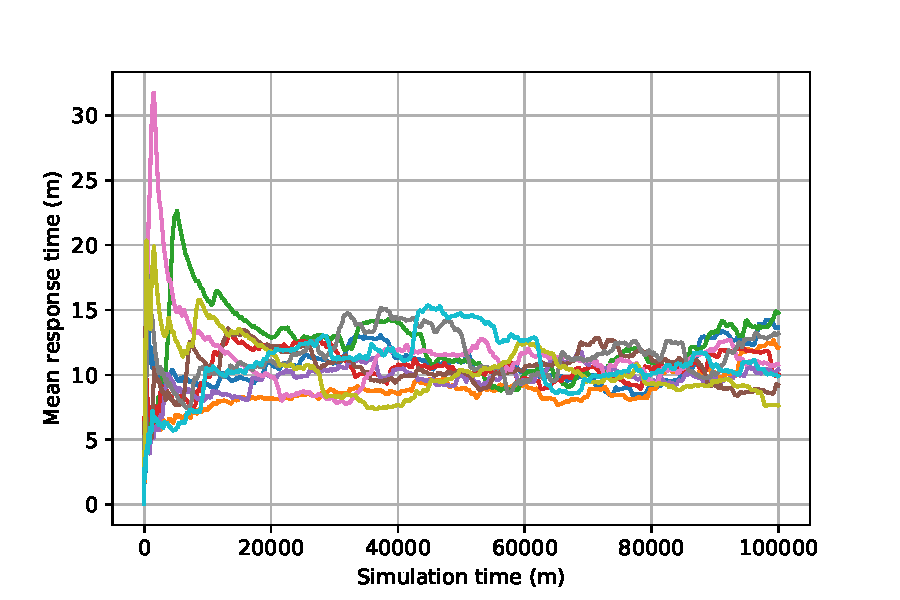
\includegraphics[width=\textwidth]{figs/warmup_definition.pdf}
  \label{fig:warmup}
\end{minipage}

After having chosen the warm-up period, the simulation time was chosen as to have both a high level of accuracy and a small execution time. The value of 500000m has hence been chosen since it provides a confidence interval around 2\% with 90\% confidence in the above worst-case scenario.

\subsection{Steady-state analyses}

\subsubsection{2kr analysis}\label{sec:2kr}
In order to grasp the factors contribution to the customers experience, we computed a number of 2$^k$r (r = 5) factorial analysis. In these analyses, we took into 
consideratione the following factors in the FIFO kitchen and exponential service and inter-arrival rates scenario: 
\begin{itemize}
  \item A = normal customers rate (vip rate is set as to keep the total rate constant) $[0.1, 1.2]$
  \item B = odds of an order being a Compound one $[0.1, 0.3]$
  \item C = kitchen Rate $[0.45, 0.6]$
  \item D = cashier Rate $[1.5, 2]$
\end{itemize}
Please note that A is, in reality, a measure of the numer of number customers 
over the total, ranging from ~10\% to ~90\%.

After having run the analyses, we visually checked the residuals' hypotheses for every metric through the related qqplot, scatter and lag plots. % TODO queue lengths

We analyzed all of the metrics and we found no strange behaviour. For the sake of brevity, we will only report the most interesting results we found:
\begin{itemize}
  \item the cashier rate has a negative impact (-0.159, with an explained 92\%
   variability) on the advantage of VIP customers 
    on normal customers since an increase of it implies lower queueing and thus 
    a more ``equal'' waiting time between VIP and normal users.
  \item parameter A has a negative contribution on the advantage of VIP       
    customers on normal customers. This is somewhat unexpected since you would 
    expect the VIP advantage to increase if fewer VIP customers are present.
    However, this results highlights the phenomenon of ``quasi-starvation''
    happening to normal customer with an high number of VIP customers. In fact:
      \begin{itemize}
        \item Many VIP users, few Normal users: VIP customers experience longer 
          waiting times (than if they were fewer), while normal users experience huge waiting times due to too many VIP arrivals jumping in queue in front of them.
        \item Few VIP users, many Normal users: VIP customers are serviced very fast, but normal user are no more ``starvated'' by VIPs. The Normal response time has lowered much more from the previous case, compared to the Vip response time, leading to a lower the simpleResponseTimeRatio.
        \item the cashier rate has a negligible influence on the kitchen queue length. This phenomenon will be further investigated in \cref{sec:cashier_no_infl}.
      \end{itemize}
\end{itemize} % si può tagliare ancora se serve

% % OLD 2kr
% \subsection{Fifo Scenario}

% \subsubsection{simpleResponseTimeRatio}

% \begin{center}
\begin{tabular}{|c|c|c|c|c|}
\cline{2-5}
\multicolumn{1}{c|}{} & q & SSx & Variation & Confidence Interval \\
\hline
A&-0.0682&0.373&10.41\% &(-0.0697, -0.0668) \\
\hline
B&0.115&1.06&29.66\% &(0.114, 0.117) \\
\hline
AB&0.0155&0.0193&0.54\% &(0.0141, 0.017) \\
\hline
C&-0.0457&0.167&4.67\% &(-0.0472, -0.0443) \\
\hline
AC&-0.00547&0.00239&0.07\% &(-0.00692, -0.00402) \\
\hline
BC&-0.0576&0.266&7.42\% &(-0.0591, -0.0562) \\
\hline
ABC&-0.00591&0.00279&0.08\% &(-0.00736, -0.00445) \\
\hline
D&-0.122&1.18&33.00\% &(-0.123, -0.12) \\
\hline
AD&0.0166&0.0221&0.62\% &(0.0152, 0.0181) \\
\hline
BD&0.0696&0.388&10.84\% &(0.0682, 0.0711) \\
\hline
ABD&-0.0124&0.0123&0.34\% &(-0.0138, -0.0109) \\
\hline
CD&-0.0252&0.051&1.42\% &(-0.0267, -0.0238) \\
\hline
ACD&0.00153&0.000186&0.01\% &(7.26e-05, 0.00298) \\
\hline
BCD&-0.0185&0.0274&0.77\% &(-0.02, -0.017) \\
\hline
ABCD&0.0047&0.00177&0.05\% &(0.00325, 0.00615) \\
\hline
Errors& &0.00388&0.11\% & \\
\hline
\end{tabular}
\end{center}

 
% There's no particular interplay occurring between factors, we can clearly see that the simpleResponseTimeRatio depends on:
% \begin{itemize}
%     \item The main reason why VIP users are privileged is due to the queueing of orders, if there's no queue the difference of Normal and Vip response times are negligible. This is exactly why the cashier rate has a negative contribution: with the increase of this factor there's less queueing and thus when a new normal order comes chances are that there will be no Vip users in queue so it can be served immediately.
%   \item The ratio between the amount of VIP and Normal users (A) has a negative contribution, this is a little bit unexpected. The reason has a connection with the starvation of Normal users. Let's try to break it up in two cases: 

% \end{itemize}

% %\begin{center}
\begin{tabular}{|c|c|c|c|c|}
\cline{2-5}
\multicolumn{1}{c|}{} & q & SSx & Variation & Confidence Interval \\
\hline
A&-0.0682&0.373&10.41\% &(-0.0697, -0.0668) \\
\hline
B&0.115&1.06&29.66\% &(0.114, 0.117) \\
\hline
AB&0.0155&0.0193&0.54\% &(0.0141, 0.017) \\
\hline
C&-0.0457&0.167&4.67\% &(-0.0472, -0.0443) \\
\hline
AC&-0.00547&0.00239&0.07\% &(-0.00692, -0.00402) \\
\hline
BC&-0.0576&0.266&7.42\% &(-0.0591, -0.0562) \\
\hline
ABC&-0.00591&0.00279&0.08\% &(-0.00736, -0.00445) \\
\hline
D&-0.122&1.18&33.00\% &(-0.123, -0.12) \\
\hline
AD&0.0166&0.0221&0.62\% &(0.0152, 0.0181) \\
\hline
BD&0.0696&0.388&10.84\% &(0.0682, 0.0711) \\
\hline
ABD&-0.0124&0.0123&0.34\% &(-0.0138, -0.0109) \\
\hline
CD&-0.0252&0.051&1.42\% &(-0.0267, -0.0238) \\
\hline
ACD&0.00153&0.000186&0.01\% &(7.26e-05, 0.00298) \\
\hline
BCD&-0.0185&0.0274&0.77\% &(-0.02, -0.017) \\
\hline
ABCD&0.0047&0.00177&0.05\% &(0.00325, 0.00615) \\
\hline
Errors& &0.00388&0.11\% & \\
\hline
\end{tabular}
\end{center}
 TODO path to compoundResponseTimeRatio FIFO

% %da decidere se inserire anche questa statistica
% \subsubsection{cashierVipQueueLength}

% \begin{center}
\begin{tabular}{|c|c|c|c|c|}
\cline{2-5}
\multicolumn{1}{c|}{} & q & SSx & Variation & Confidence Interval \\
\hline
A&-0.0682&0.373&10.41\% &(-0.0697, -0.0668) \\
\hline
B&0.115&1.06&29.66\% &(0.114, 0.117) \\
\hline
AB&0.0155&0.0193&0.54\% &(0.0141, 0.017) \\
\hline
C&-0.0457&0.167&4.67\% &(-0.0472, -0.0443) \\
\hline
AC&-0.00547&0.00239&0.07\% &(-0.00692, -0.00402) \\
\hline
BC&-0.0576&0.266&7.42\% &(-0.0591, -0.0562) \\
\hline
ABC&-0.00591&0.00279&0.08\% &(-0.00736, -0.00445) \\
\hline
D&-0.122&1.18&33.00\% &(-0.123, -0.12) \\
\hline
AD&0.0166&0.0221&0.62\% &(0.0152, 0.0181) \\
\hline
BD&0.0696&0.388&10.84\% &(0.0682, 0.0711) \\
\hline
ABD&-0.0124&0.0123&0.34\% &(-0.0138, -0.0109) \\
\hline
CD&-0.0252&0.051&1.42\% &(-0.0267, -0.0238) \\
\hline
ACD&0.00153&0.000186&0.01\% &(7.26e-05, 0.00298) \\
\hline
BCD&-0.0185&0.0274&0.77\% &(-0.02, -0.017) \\
\hline
ABCD&0.0047&0.00177&0.05\% &(0.00325, 0.00615) \\
\hline
Errors& &0.00388&0.11\% & \\
\hline
\end{tabular}
\end{center}

% We can observe that:
% \begin{itemize}
%     \item if the Vip arrival rate decreases (factor A increases) the VIP queue length will also decrease accordingly.
%     \item by increasing the cashier rate Vip queue length will also decrease.
%     \item Here we can also see an interesting interplay by factor A and D, meaning that a good portion of the variation is explained by the interaction of those factors.
% \end{itemize}

% \subsubsection{cashierNormalQueueLength}
% \begin{center}
\begin{tabular}{|c|c|c|c|c|}
\cline{2-5}
\multicolumn{1}{c|}{} & q & SSx & Variation & Confidence Interval \\
\hline
A&-0.0682&0.373&10.41\% &(-0.0697, -0.0668) \\
\hline
B&0.115&1.06&29.66\% &(0.114, 0.117) \\
\hline
AB&0.0155&0.0193&0.54\% &(0.0141, 0.017) \\
\hline
C&-0.0457&0.167&4.67\% &(-0.0472, -0.0443) \\
\hline
AC&-0.00547&0.00239&0.07\% &(-0.00692, -0.00402) \\
\hline
BC&-0.0576&0.266&7.42\% &(-0.0591, -0.0562) \\
\hline
ABC&-0.00591&0.00279&0.08\% &(-0.00736, -0.00445) \\
\hline
D&-0.122&1.18&33.00\% &(-0.123, -0.12) \\
\hline
AD&0.0166&0.0221&0.62\% &(0.0152, 0.0181) \\
\hline
BD&0.0696&0.388&10.84\% &(0.0682, 0.0711) \\
\hline
ABD&-0.0124&0.0123&0.34\% &(-0.0138, -0.0109) \\
\hline
CD&-0.0252&0.051&1.42\% &(-0.0267, -0.0238) \\
\hline
ACD&0.00153&0.000186&0.01\% &(7.26e-05, 0.00298) \\
\hline
BCD&-0.0185&0.0274&0.77\% &(-0.02, -0.017) \\
\hline
ABCD&0.0047&0.00177&0.05\% &(0.00325, 0.00615) \\
\hline
Errors& &0.00388&0.11\% & \\
\hline
\end{tabular}
\end{center}


% Basically all the observation done for the cashierVipQueueLength remains with minor changes. We can observe that now factor A has a positive contribution, this was to be expected because by increasing factor A we increase the Normal arrival rate meaning that new Normal orders are subject to longer queue.

% \subsubsection{kitchenQueueLength}

% \begin{center}
\begin{tabular}{|c|c|c|c|c|}
\cline{2-5}
\multicolumn{1}{c|}{} & q & SSx & Variation & Confidence Interval \\
\hline
A&-0.0682&0.373&10.41\% &(-0.0697, -0.0668) \\
\hline
B&0.115&1.06&29.66\% &(0.114, 0.117) \\
\hline
AB&0.0155&0.0193&0.54\% &(0.0141, 0.017) \\
\hline
C&-0.0457&0.167&4.67\% &(-0.0472, -0.0443) \\
\hline
AC&-0.00547&0.00239&0.07\% &(-0.00692, -0.00402) \\
\hline
BC&-0.0576&0.266&7.42\% &(-0.0591, -0.0562) \\
\hline
ABC&-0.00591&0.00279&0.08\% &(-0.00736, -0.00445) \\
\hline
D&-0.122&1.18&33.00\% &(-0.123, -0.12) \\
\hline
AD&0.0166&0.0221&0.62\% &(0.0152, 0.0181) \\
\hline
BD&0.0696&0.388&10.84\% &(0.0682, 0.0711) \\
\hline
ABD&-0.0124&0.0123&0.34\% &(-0.0138, -0.0109) \\
\hline
CD&-0.0252&0.051&1.42\% &(-0.0267, -0.0238) \\
\hline
ACD&0.00153&0.000186&0.01\% &(7.26e-05, 0.00298) \\
\hline
BCD&-0.0185&0.0274&0.77\% &(-0.02, -0.017) \\
\hline
ABCD&0.0047&0.00177&0.05\% &(0.00325, 0.00615) \\
\hline
Errors& &0.00388&0.11\% & \\
\hline
\end{tabular}
\end{center}


% In this particular scenario the kitchen has no priority queue. This means that all the orders coming from the cashier are treated in the same way, even if they are VIP. Of course, by that, we can expect that factor A would not bring any contribution to the variation and it's exactly what we can see from the results. Instead:
% \begin{itemize}
%     \item factor B has high positive contribution. By increasing it (probability of compound orders increase) we can expect longer queue.
%     \item of course by increasing factor C (kitchen rate) we can expect shorter queue in the kitchen.
%     \item Here we can also see an interesting interplay by factor A and D, meaning that a good portion of the variation is explained by the interaction of those factors.
% \end{itemize}

% \subsection{Priority Scenario}

% For what concern the cashier part of the system, all the observations done in the Fifo scenario still holds. In fact we can see that all the results are exactly the same, so we will not discuss this case any further.

% %\input{Analysis\Fifo\} TODO path to compoundResponseTimeRatio Priority

% %spiegazione

% \subsubsection{kitchenVipQueueLength}
% \begin{center}
\begin{tabular}{|c|c|c|c|c|}
\cline{2-5}
\multicolumn{1}{c|}{} & q & SSx & Variation & Confidence Interval \\
\hline
A&-0.0682&0.373&10.41\% &(-0.0697, -0.0668) \\
\hline
B&0.115&1.06&29.66\% &(0.114, 0.117) \\
\hline
AB&0.0155&0.0193&0.54\% &(0.0141, 0.017) \\
\hline
C&-0.0457&0.167&4.67\% &(-0.0472, -0.0443) \\
\hline
AC&-0.00547&0.00239&0.07\% &(-0.00692, -0.00402) \\
\hline
BC&-0.0576&0.266&7.42\% &(-0.0591, -0.0562) \\
\hline
ABC&-0.00591&0.00279&0.08\% &(-0.00736, -0.00445) \\
\hline
D&-0.122&1.18&33.00\% &(-0.123, -0.12) \\
\hline
AD&0.0166&0.0221&0.62\% &(0.0152, 0.0181) \\
\hline
BD&0.0696&0.388&10.84\% &(0.0682, 0.0711) \\
\hline
ABD&-0.0124&0.0123&0.34\% &(-0.0138, -0.0109) \\
\hline
CD&-0.0252&0.051&1.42\% &(-0.0267, -0.0238) \\
\hline
ACD&0.00153&0.000186&0.01\% &(7.26e-05, 0.00298) \\
\hline
BCD&-0.0185&0.0274&0.77\% &(-0.02, -0.017) \\
\hline
ABCD&0.0047&0.00177&0.05\% &(0.00325, 0.00615) \\
\hline
Errors& &0.00388&0.11\% & \\
\hline
\end{tabular}
\end{center}


% \begin{itemize}
%     \item by increasing factor A (Normal Arrival Rate increases, Vip arrival Rate decreases) the VIP queue length tends to decrease.
%     \item by increasing factor B (probability of compound orders), the total inter-arrival rate of the kitchen increases too so new orders are more subject to queueing.
%     \item of course, by increasing the Kitchen Rate (factor C) the length of VIP Queue length decreases.
%     \item of course by being a Pasta system (no orders are created or destroyed inside the system), the inter-arrival rate of the cashier is also the inter-departure rate and, by that, we can be sure that the cashier rate (factors D) brings no contribution to the Normal Queue Length in the kitchen. %TODO da controllare
% \end{itemize}

% \subsubsection{kitchenNormalQueueLength}
% \begin{center}
\begin{tabular}{|c|c|c|c|c|}
\cline{2-5}
\multicolumn{1}{c|}{} & q & SSx & Variation & Confidence Interval \\
\hline
A&-0.0682&0.373&10.41\% &(-0.0697, -0.0668) \\
\hline
B&0.115&1.06&29.66\% &(0.114, 0.117) \\
\hline
AB&0.0155&0.0193&0.54\% &(0.0141, 0.017) \\
\hline
C&-0.0457&0.167&4.67\% &(-0.0472, -0.0443) \\
\hline
AC&-0.00547&0.00239&0.07\% &(-0.00692, -0.00402) \\
\hline
BC&-0.0576&0.266&7.42\% &(-0.0591, -0.0562) \\
\hline
ABC&-0.00591&0.00279&0.08\% &(-0.00736, -0.00445) \\
\hline
D&-0.122&1.18&33.00\% &(-0.123, -0.12) \\
\hline
AD&0.0166&0.0221&0.62\% &(0.0152, 0.0181) \\
\hline
BD&0.0696&0.388&10.84\% &(0.0682, 0.0711) \\
\hline
ABD&-0.0124&0.0123&0.34\% &(-0.0138, -0.0109) \\
\hline
CD&-0.0252&0.051&1.42\% &(-0.0267, -0.0238) \\
\hline
ACD&0.00153&0.000186&0.01\% &(7.26e-05, 0.00298) \\
\hline
BCD&-0.0185&0.0274&0.77\% &(-0.02, -0.017) \\
\hline
ABCD&0.0047&0.00177&0.05\% &(0.00325, 0.00615) \\
\hline
Errors& &0.00388&0.11\% & \\
\hline
\end{tabular}
\end{center}


% We can observe that:
% \begin{itemize}
%     \item by increasing factor A (Normal Arrival Rate increases) the Normal queue length tends to increase too.
%     \item by increasing factor B (probability of compound orders), the total inter-arrival rate of the kitchen increases too so new orders are more subject to queueing.
%     \item of course, by increasing the Kitchen Rate (factor C) the length of Normal Queue length decreases.
%     \item of course by being a Pasta system (no orders are created or destroyed inside the system), the inter-arrival rate of the cashier is also the inter-departure rate and, by that, we can be sure that the cashier rate brings no contribution to the Normal Queue Length in the kitchen. %TODO da controllare
%     \item all the interplays bring negligible contributions apart from the BC one which should be taken into consideration when tuning the system. %TODO dacontrollare
% \end{itemize}

\subsubsection{Kitchen Queue Comparison}

Now we want to assess if enforcing a priority queue also in the kitchen brings any perks. In order to get that results we observe the trajectories of the \emph{compoundResponseTimeRatio} statistic (i.e. the advantage of being a VIP customer over a normal customer when the order is compound) in both cases, fifo queue and priority queue, varying the ratio of compound orders.

\begin{figure}[h!]
    \centering
    \begin{minipage}{0.48\textwidth}
      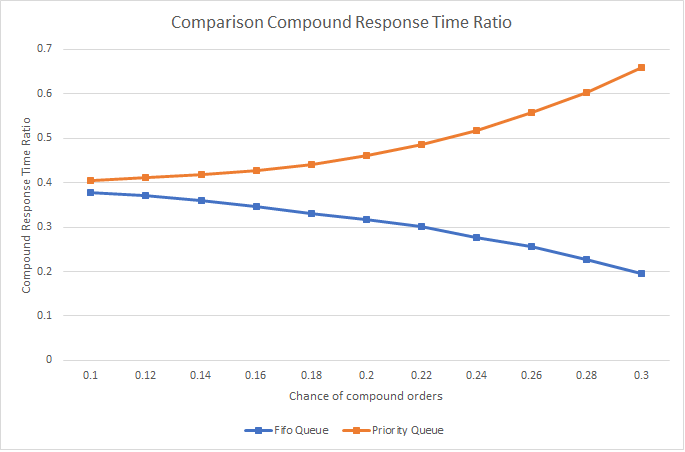
\includegraphics[width=\textwidth]{figs/comparisonQueue.png}
      \caption{} % Explain used configuration
      \label{}
    \end{minipage}\hspace{0.03\textwidth}
    \begin{minipage}{0.48\textwidth}
      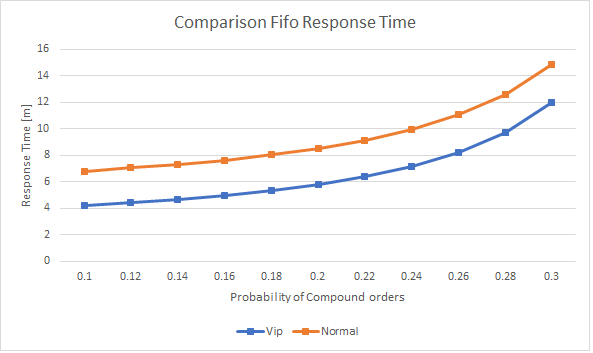
\includegraphics[width=\textwidth]{figs/comparisonFifoKitchen.png}
      \caption{} % Explain used configuration
      \label{}
    \end{minipage}
\end{figure}

% Refer to figures using /cref{} 
We can clearly see that by increasing the number of compound orders, in the fifo case, Vip users tend to lose the ``advantage'' obtained during the cashier service. So, indeed, by using a priority queue in kitchen we can provide an even more privileged service. But is it necessary? Of course not, it depends on the type of service that the Bar Administrator strive to get. In fact we see that even without using a priority queue in the kitchen, the advantage obtained during the cashier service is enough to let Vip user have some benefits (around 2m) even in case of compound orders:

% Sarebbe interessante anche un plot della differenza dei response time tra vip e normal nei due casi, ovvero R_FIFO - R_PRIO per entrambi, e vedere, per ogni minuto guadagnato dal vip, quanto deve aspettare il normal in più

\subsubsection{System Response to different Workloads}

\begin{figure}[h!]
  \begin{minipage}{0.48\textwidth}
    \centering
    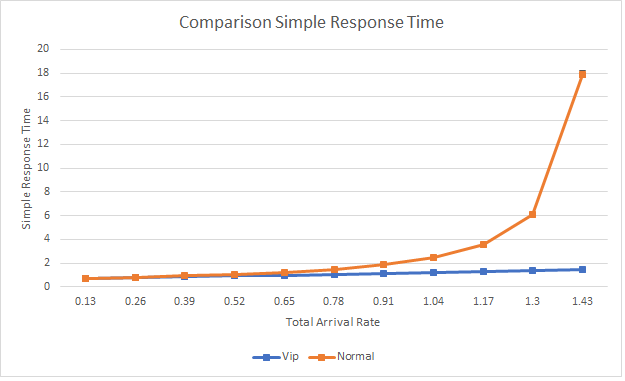
\includegraphics[width=\textwidth]{figs/workloadSimple.png}
    \caption{}  % Explain used configuration
    \label{}
  \end{minipage}\hspace{0.03\textwidth}
  \begin{minipage}{0.48\textwidth}
    \centering
    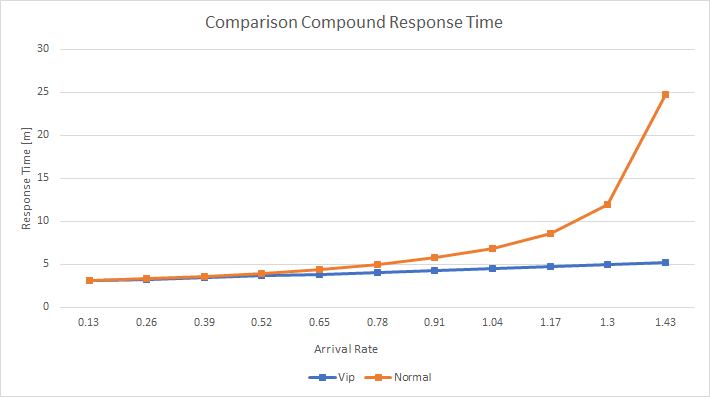
\includegraphics[width=\textwidth]{figs/workloadCompound.png}
    \caption{} % Explain used configuration
    \label{}
  \end{minipage}
\end{figure}

Note that the Inter-Arrival rate for the kitchen with this configuration is actually 0.2 * "value showed in the x axis". We kept those numbers only to let the reader catch the similarities with the previous graph. %TODO da controllare
% Più commenti tipo "il bar risponde bene finchè l'arrival rate è sotto a 1.3 poi esplode"

\subsubsection{Vip Rate study}

\begin{figure}[h!]
  \begin{minipage}{0.48\textwidth}
    \centering
    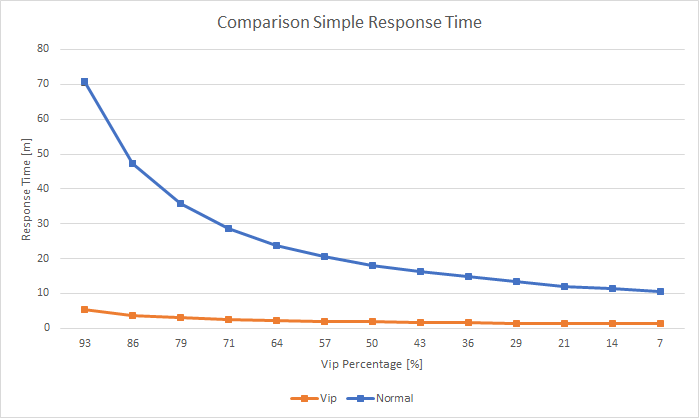
\includegraphics[width=\textwidth]{figs/comparisonSimpleResponseTime.png}
    \caption{} % Explain used configuration
    \label{}
  \end{minipage}\hspace{0.03\textwidth}
  \begin{minipage}{0.48\textwidth}
    \centering
    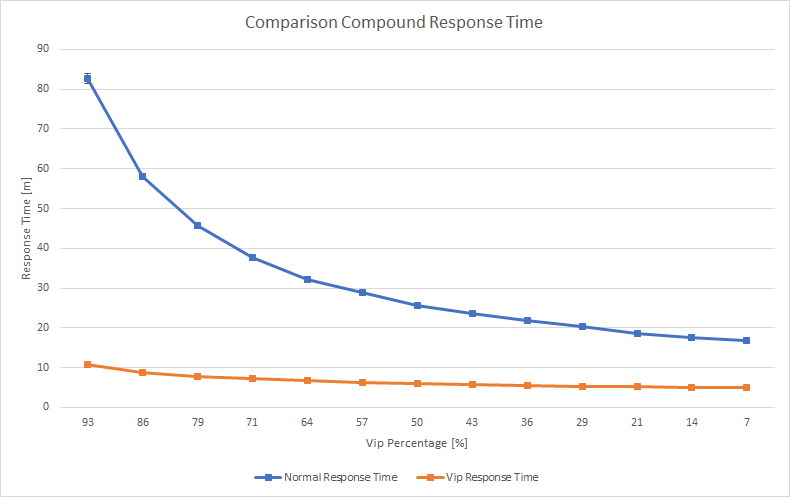
\includegraphics[width=\textwidth]{figs/comparisonCompoundResponseTime.png}
    \caption{} % Explain used configuration
    \label{}
  \end{minipage}
\end{figure}

One thing that should be taken into consideration when fine-tuning the system is the amount of allowed VIP customers. Of course if all users were VIP, they would gain little to no benefit and chances are that the few normal customers that arrive will experience a vary bad service. Therefore, it is interesting to study the response of the system at varying percentages of VIP customers in order to find an ``optimal'' value, i.e. one such that VIP benefits are preserved and normal customers are served in a reasonable time. Such study was carried out with a full factorial analysis, varying the percentage of VIP customers.

By changing only the percentage of VIP users we can set a reasonable response time for Normal user (we opted for 15m) and establish the optimal percentage of Vip users which we found it to be between 10\% and 30\%.

We can also plot the simpleResponseTimeRatio with the same configuration and ensure that, in fact, Vip users are at least 80\% faster than Normal users in that range.

All the above can be repeated for the kitchen in the Priority case to get similar results. In fact we can expect a fairly reasonable response time from normal users in the same range:

\begin{figure}[H]
    \centering
    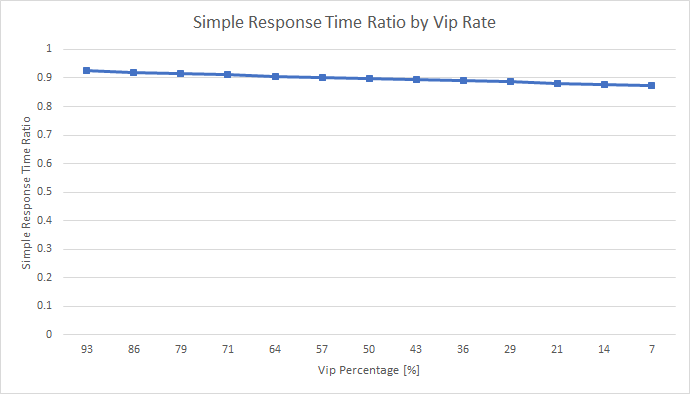
\includegraphics[width=0.75\textwidth]{figs/simpleResponseTimeRatio.png} % QUALCOSA NON MI TORNA
\end{figure}

\subsubsection{Relationship between service rates proportion and queue lengths}
\label{sec:cashier_no_infl}

In this section we will investigate the relationship between the proportion of the service rates and queue lengths. First of all, let's notice that the queue at the cashier is by no means influenced by the rate of the cashier, therefore we will just look at the behaviour of the kitchen queue in both fifo and priority queueing strategies.

\begin{figure}
  \begin{minipage}{0.32\textwidth}
    \centering
    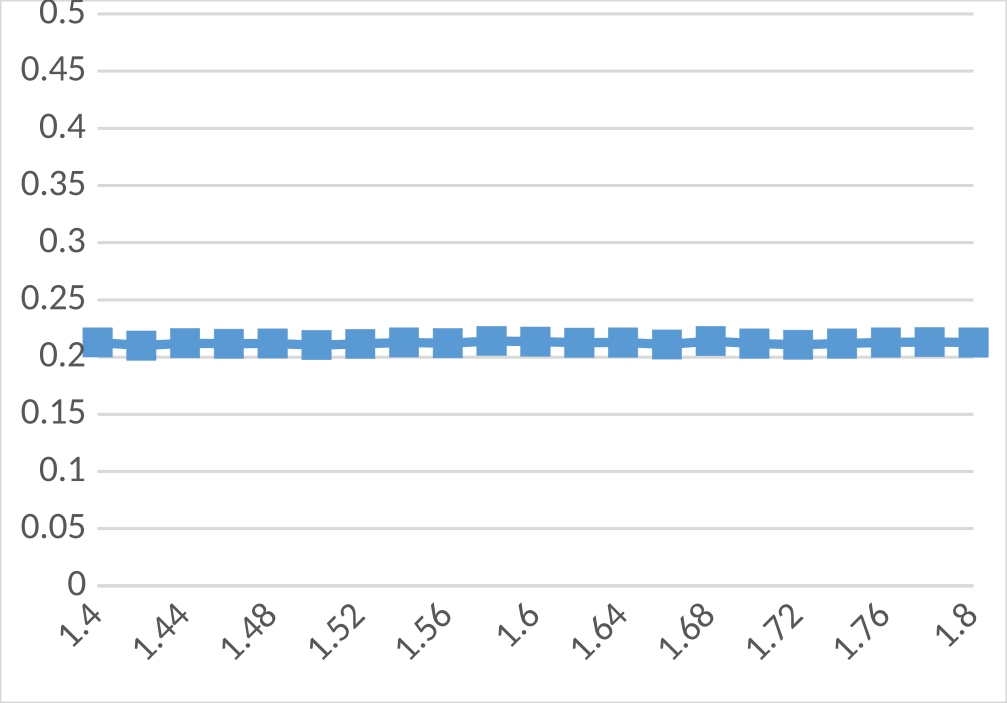
\includegraphics[width=\textwidth]{figs/inv_ql_fifo.png}
    (a)
  \end{minipage}\hspace{0.01\textwidth}
  \begin{minipage}{0.32\textwidth}
    \centering
    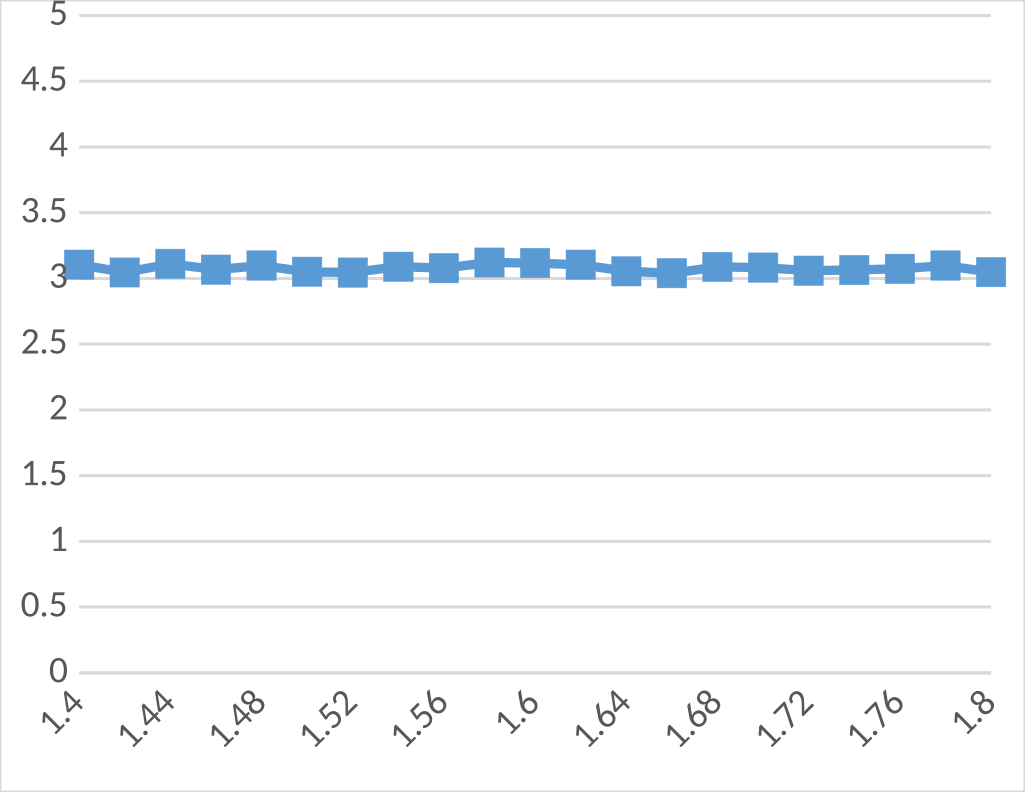
\includegraphics[width=\textwidth]{figs/inv_ql_normal.png}
    (b)
  \end{minipage}\hspace{0.01\textwidth}
  \begin{minipage}{0.32\textwidth}
    \centering
    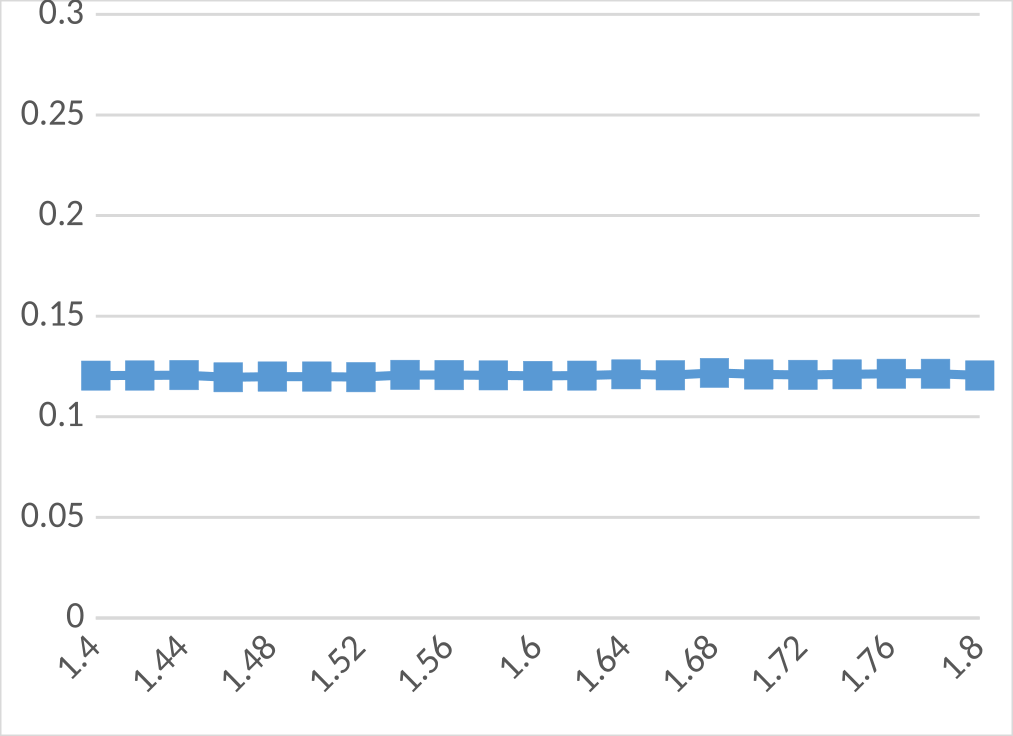
\includegraphics[width=\textwidth]{figs/inv_ql_vip.png}
    (c)
  \end{minipage}
  \caption{Kitchen queue length as a function of the cashier service rate in the FIFO (a) and priority (b: normal queue; c: vip queue). 
  $r=30,\lambda_N=1,\lambda_V=0.2,\pi_C=0.2,\mu_K=0.3,\mu_C=\{1.4..1.8 \text{ step } 0.02\}$.}
  \label{fig:inv_ql}
\end{figure}

In \cref{sec:2kr} we showed how the kitchen mean queue length was not influenced by the cashier rate and \cref{fig:inv_ql} just confirms the above result. Furthermore, recall that the same result was obtained also in the mathematical model for the FIFO case.

\subsection{``Business day'' analysis}
After having studied the system response at the steady state, we decided to observe it also in a business day. We used the multipliers in \cref{fig:bd:mul} to vary the arrival rate throughout the day so that to have peaks during meal times. In the following section, each scenario has been repeated 100 times and obtained confidence intervals are shown in the plots.

\begin{figure}
  \begin{minipage}{0.48\textwidth}
    \centering
    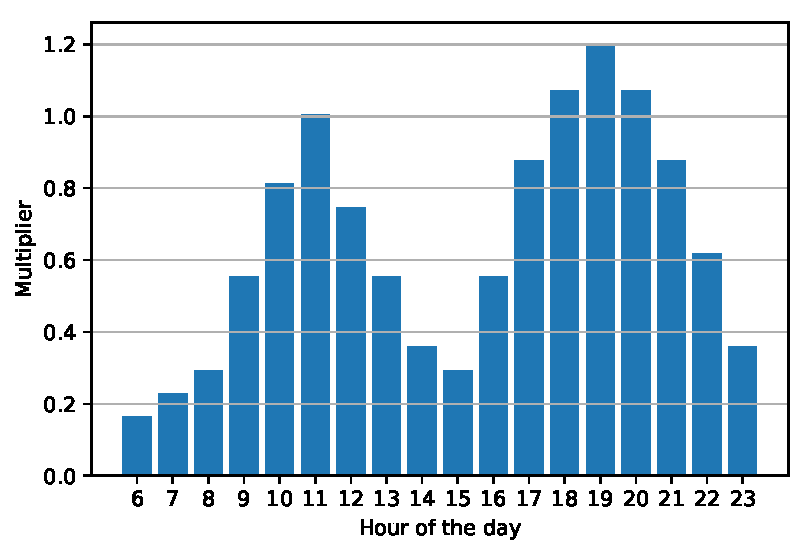
\includegraphics[width=\textwidth]{figs/business_day/input_bd.pdf}
    \caption{Multipliers used to modify the average arrival rate per business hour.}
    \label{fig:bd:mul}
  \end{minipage}\hspace{0.03\textwidth}
  \begin{minipage}{0.48\textwidth}
    \centering
    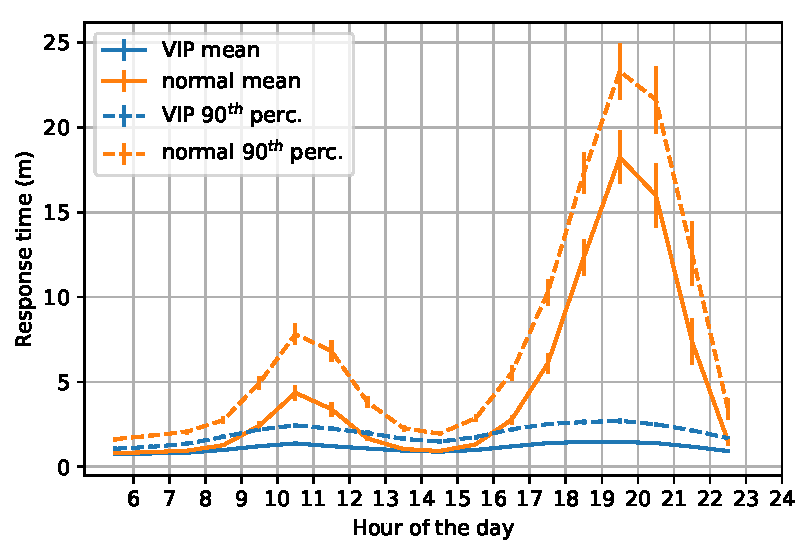
\includegraphics[width=\textwidth]{figs/business_day/vip_vs_normal_simple.pdf}
    \caption{Comparison of the hourly average of the response time for VIP and normal customers with simple orders in a ``normal'' business day ($\mu_C=1.5, \mu_K=0.4, \lambda_{tot,max} = 1.65, \pi_V=0.2, \pi_C=0.2$).}
    \label{fig:bd:vip_vs_norm}
  \end{minipage}
\end{figure}

\cref{fig:bd:vip_vs_norm} shows a comparison between VIP and normal customers. As expected, the VIP customers are serviced very fast and experience almost no waiting time. Furthermore, note that the mean waiting time during dinner is much higher than lunch time since, with the used configuration, during the former the arrival rate exceeds the cashier service rate, conversely to what happens in the latter.

\cref{fig:bd:var_cr,fig:bd:var_ar} show the response of the system when varying, respectively, the cashier rate and the arrival rate. Both plots highlight that a small change ($\sim 10\%$) of either rate leads to an exponential change of the response time. Thus, even a small improvement in cashier speed during peak times could lead to huge improvements in customer satisfaction.

\begin{figure}
  \begin{minipage}{0.48\textwidth}
    \centering
    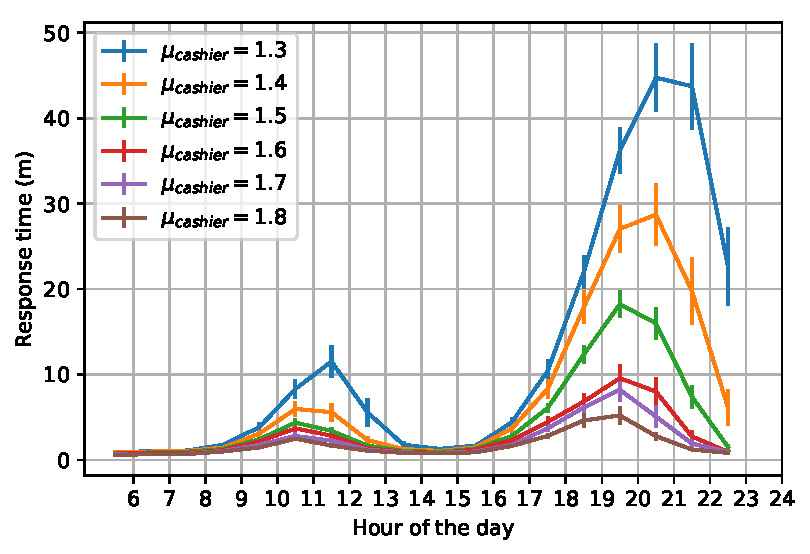
\includegraphics[width=\textwidth]{figs/business_day/varying_cashier_rate.pdf}
    \caption{Hourly average of the response time for normal-simple orders in a business day at different cashier rates ($\mu_K=0.4, \lambda_{tot,max} = 1.65, \pi_V=0.2$).}
    \label{fig:bd:var_cr}
  \end{minipage}\hspace{0.03\textwidth}
  \begin{minipage}{0.48\textwidth}
    \centering
    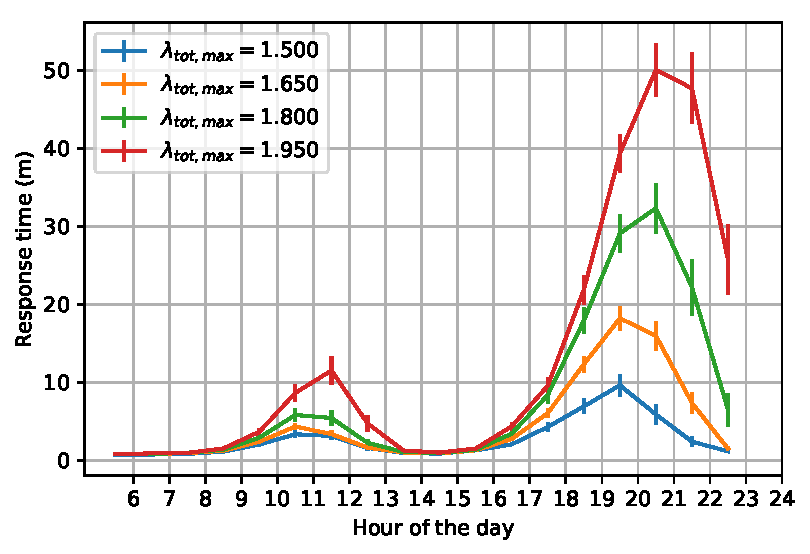
\includegraphics[width=\textwidth]{figs/business_day/varying_arrival_rate.pdf}
    \caption{Hourly average of the response time for normal-simple orders in a business day at different arrival rates ($\mu_C = 1.5, \mu_K=0.4, \pi_V=0.2$).}
    \label{fig:bd:var_ar}
  \end{minipage}
\end{figure}

\section{Conclusions}
Our study has shown how the customers' experienced waiting time is related to the factors of the systems. Obvious relationships have been confirmed, like those related to cashier and kitchen rate. 
Furthermore, we showed that, counterintuitively, the mean queue length at the kitchen is not influenced by the speed of the cashier (in the considered exponential scenario). 
We also showed that the number of VIP customers over the total can negatively impact the satisfaction of normal customers.

The possibility of introducing priority queueing also in the kitchen has been explored. On the one hand, it obviously increases the benefits of the VIP user but, on the other hand, it reduces normal customers satisfaction. The choice of its introduction should carefully weigh these two factors.

Finally, by studying a classic business day, we showed how small improvements in the cashier serving speed can have huge benefits on the overall customer experience.
